\subsection{Topologie}
\label{subsec:CR:topologie}

Pour effectuer les exp�riences de d�bit avec MPTCP, nous utilisons
principalement deux topologies (A et B).

La topologie A est inspir� du \emph{testbed} de l'article de
R. Khalili \cite{pareto2013}, voir \fig{fig:topoMPTCP:A}. Nous avons
ajout� � cette topolgoie des routeurs priv�s entre le client et le
serveur \emph{MPTCP} pour augmenter le nombre de sous-flots.

\begin{figure}[!htb]
  \begin{changemargin}{-2.0cm}{0.5cm}
    \centering
    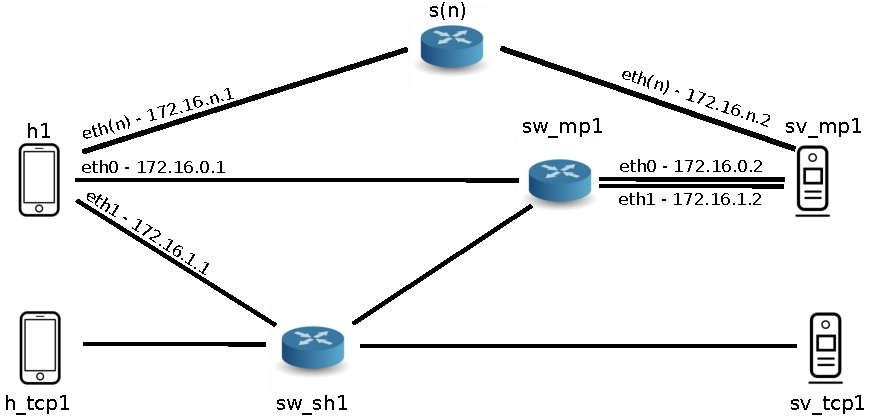
\includegraphics[width=0.7\textwidth]{../figures/mptcp_tcp/mptcp_tcp.pdf}
  \end{changemargin}
  \centering
  
  \caption{\textbf{Reproduction de la topologie de l'article de
      R. Khalili}. Le(s) \emph{switch(s)} n ne sont pr�sent(s) que si
    le nombre de sous-flot est sup�rieure � deux. Pour n sous-flots,
    il y aura cr�ation de n-2 \emph{switchs} et autant de liens
    suppl�mentaires. L'hyperviseur est connect� � tous les
    switchs. Pour se connecter via ssh aux h�tes, un \emph{switch} \og
    root \fg est cr�� et est connect� au \emph{switch} sw\_mp1 (non
    repr�sent� ici) voir utilisations CF linktobeadded.}
  \label{fig:topoMPTCP:A}
  
\end{figure}